\chapter{Introduction}

A blockchain, is a continuously growing list of records, called blocks, which
are linked and secured using cryptography. Each block typically contains a
cryptographic hash of the previous block, a time stamp and transaction data. By
design, a blockchain is immutable because of the linked structure. It is ”an open,
distributed ledger that can record transactions between two parties efficiently
and in a verifiable and permanent way” according to \citep{blockchain-def}. In
order to be used as distributed ledger, it is managed by a peer to peer
network, in which all peers/nodes follow one protocol. This protocol takes care
of messaging between these peers, and adding and validating the new blocks
formed. Once a block is added to the blockchain, the block can't be altered,
since all blocks added after will need to be changed. 

Blockchains are secure by design and exemplify a distributed computing system
with high Byzantine fault tolerance, leading to consensus in a decentralized
network.

This makes blockchains potentially suitable for the recording of events,
medical records, and other records management activities, such as identity
management, transaction processing, documenting provenance, food traceability,
and voting. \citep{blockchain-wiki} Blockchain was invented by Satoshi
Nakamoto in 2008 to serve as the public transaction ledger of the
cryptocurrency bitcoin \citep{bitcoin}. The invention of the blockchain for
bitcoin made it the first digital currency to solve the double-spending
problem without the need of trust. Blockchain networks essentially engage two
major types of actors:

\begin{enumerate}
    \item \textbf{Miners:} Mining is the process of adding transaction records
        to the public ledger. The miners, in a proof of work blockchain, solve a
        computationally difficult problem in order to add a block to the ledger.
        In bitcoin, this problem is to solve for a number (nonce) \citep{nonce} that when
        hashed with the block data must start with a certain number of zeroes.
        This number of zeroes is termed the difficulty of the network. The miner
        who successfully adds a block to the ledger is rewarded with a block
        reward along with the fee on all transactions included in the block. The
        miners, therefore have incentive in computing the hash for the next
        block and propagating it to the network so that their block is accepted.
        In order to mine these computationally expensive hashes and propagate
        them through the network, miners invest heavily into high grade
        infrastructure, bandwidth for the node and the electricity costs of
        running the mentioned hardware.

    \item \textbf{Propagation Nodes:} These nodes are voluntary nodes on the
        network that help in propagation of the blocks and transactions.
        Propagation nodes are of 2 types:

        \begin{enumerate}
            \item \textbf{Full Nodes:}
                These nodes help in propagating the complete blocks and fulfill
                all requests. In addition to propagating the blocks, it also
                verifies and validates the transactions by checking its inputs
                and outputs. They validate whether there is a double spend on
                the transaction by checking a complete history of the
                transaction. They also verify the signatures of the witnesses.
                In order to validate and serve all requests, these blocks store
                the complete copy of the blockchain.

            \item \textbf{Light Nodes/SPV (Simplified Payment Verification):} 
                These nodes are lightweight nodes that run on machines with
                less computational power and less storage. They also validate
                the block but not by checking the transactions in depth, but
                they do so by checking their merkle proofs.  That is basically
                hashing all the transaction hashes together to see if the
                merkle root \citep{invest-merkle} present in the block header
                is what they get after hashing all their transactions. In order
                to do so, the SPV wallets only need the header of all blocks
                included in the chain and the merkle proofs. Therefore, these
                nodes do not store a copy of the blockchain and hence don’t
                propagate complete blocks. These are often run on Raspberry Pis
                or mobile wallets. 

        \end{enumerate}

\end{enumerate}

The Dash network \citep{dash-whitepaper} employs an additional 2nd layer protocol, commonly referred to
as the \textbf{Masternode} layer.


\begin{enumerate}

    \item \textbf{Masternode:}
        These nodes are full nodes which aim to help the
        Dash blockchain network by providing services and, in return, get
        awarded by sharing a portion of the block reward with miners. The
        requirements for a full node to be a masternode are as follows:

        \begin{enumerate}
            \item The node at all times should have a 1000 dash in its wallet.
            \item The node should run a high bandwidth connection. The current
                requirement is 1 Gigabit per second.
            \item The node should run significant memory (RAM), in order to store
                the transaction set in memory for faster validation. It is
                currently 4GB but might increase based on future needs.  
        \end{enumerate}

\end{enumerate}

In order for the blockchain network to run securely and all the consensus rules
be enforced, it is important that the network contains a significant number of
full nodes and help verifying transactions and propagating complete block data.
The current bitcoin network runs 10,000 nodes approximately. 

As the blockchain decentralized network grows larger or the number of transactions on the network, the
network runs into issues relating to scalability that are explained below.


\section{Scalability Challenges with blockchains}

\subsection{Challenge: Throughput}
The block interval \citep{interval} in a blockchain network is controlled by the
mining difficulty \citep{difficulty}, which approximates to 2 minutes 30 seconds in Dash network,
and lives in the neighbourhood of 10 minutes in the bitcoin network. In the bitcoin network, the mining
difficulty is adjusted every 2016 blocks in order to get it closer to the above
mentioned intervals. The block size was initially not constrained. However, it
was later capped to 1MB 
 in 2010 \cite{controversy}. The average size of transaction on the bitcoin
network is ~500 bytes. The maximum number of transactions that can be packed
inside a block is dependent on the transaction sizes for that block, however
approximating 500 bytes a transaction, the throughput is close to 3.5
transactions per second. In the bitcoin blockchain network, it is seen that
with a mixed transaction size, the network roughly has a throughput of 3-7 
transactions per second \citep{trees-not-chains}.

Transaction sizes depend on three variables :

\begin{enumerate}
    \item List of inputs
    \item List of outputs
    \item A list of witnesses, that is one per each input and is dependent on a
        flag which if set to 0 indicates no witness.
\end{enumerate}

Majority transactions, based on the data provided by block explorers, happen
between two peers resulting in 1 input and 2 outputs along with 2 witnesses
therefore resulting in an almost static transaction size. This results in a
linear throughput increase with the increase in block size.

Public blockchains, seeing this limitation on throughput, have been slowly
forking over to larger block sizes. Dash currently has a 2MB block size limit
within a ~2.5 minute block interval. Bitcoin Cash over the years has slowly forked the
blockchain multiple times to increase the block limit to 32MB. \citep{btc-forks} lists all forks that happened with bitcoin.


\subsection{Challenge: Validation of large blocks}

As block size gets bigger, validation of individual transactions ( a 1GB block
may have over a million transactions ), 2 million taking average transaction
size to be 500 bytes,  becomes a challenge for personal computers or Raspberry
Pis that are running full nodes on the network. One of the key reasons for this
challenge is that although all clients employ infrastructure with multiple
threads, the blockchain code does not make use of threads at its full
potential. Recent research at Stanford \cite{youtube-stan} shows that even though a gigabyte block
may be propagated in the block interval constraint, it will be hard to validate
the number of transactions. This resulted in the changing the implementation of
Bitcoin Cash cryptocurrency to handle a large number of threads in order to
increase the performance of the software. 

\subsection{Challenge: Relay of large blocks}

\begin{figure}
    \captionsetup{justification=centering}
    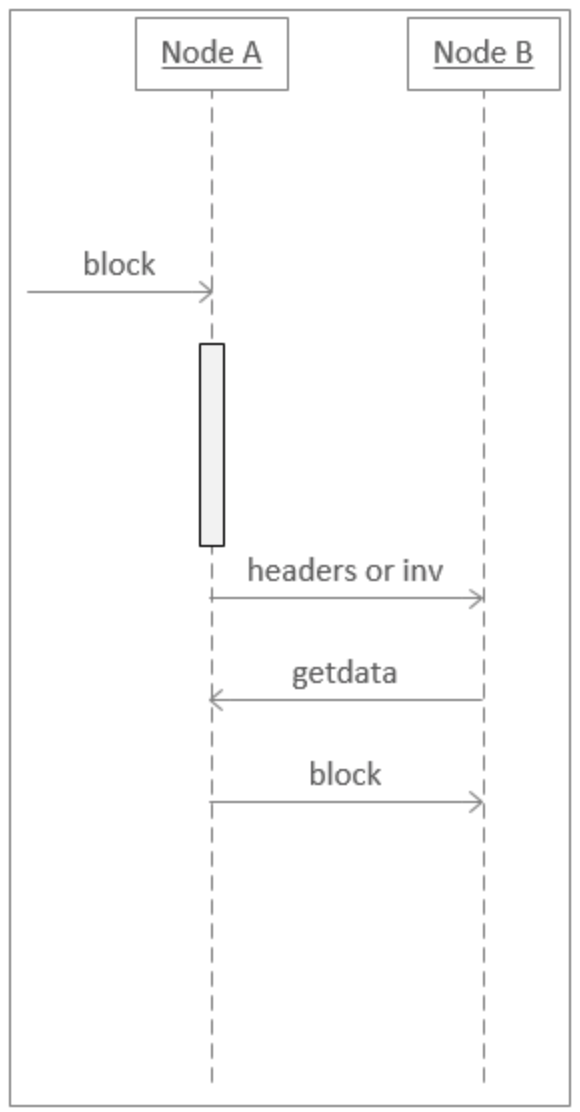
\includegraphics[width=.3\columnwidth, height=.4\columnwidth]{files/traditional.png}
     \centering
     \caption{Traditional Relay}
     \label{image: traditional}
\end{figure}

Block relay (\ref{image: traditional}) on the blockchain network uses a gossip
protocol in which  a node relays the newly heard blocks to its peers which is
approximately in the neighbourhood of 8-10 peers. This information is relayed
using a series of messages. On hearing about a new block, the first node
validates the complete block and then advertises the block its peers using an \texttt{inv}(Inventory
message, which is a 64 byte hash of the received block). If the peer on the
other side hasn’t heard of this 64 byte hash, it sends a \texttt{getdata} message ( 36
bytes ) to the first peer. In response to the \texttt{getdata} message, the second peer
now transmits the whole block to the first peer. This is the size of a full
block (current block size agreed upon by the network).

As the block size increases on the network, the last message (\texttt{getdata}) relay is
bound on the upstream bandwidth of the second peer, therefore slowing down the
propagation of blocks through the network.

Miners on the network although receive a transaction fee on adding a transaction
to the block, a major portion of their revenue come from the block reward. If
the miners are not able to propagate their blocks to the network, they lose
the block reward and with that their potential profits. The block that was mined correctly but was still not added to the
blockchain is referred to as an orphan block. This leads the miners to either
mine smaller blocks (less revenue because of less transactions) or not mine at
all. The former leads to a lower throughput and the latter leads to risks of
Centralization since only a handful a miners can afford to relay larger blocks because of high bandwidth requirements.

\section{Existing Solutions}

In the recent years, the solutions to speed up propagation process have aimed at
reducing the payload of the block. In the gossip protocol, transactions are
relayed in the network using the same process as of blocks. Every transaction
that happens on a node, is broadcasted to all its peers using an inventory
message(\texttt{inv}) that is followed by a \texttt{getdata} and a transaction data transmission,
if required. Since this data has already been transferred across the network,
there was an opportunity to send only the information required to propagate the
block. That involves a metadata of all the transactions and the full
transactions that have not already been transmitted to the requesting peer. This
led to developing three different solutions that manage to send a significantly
smaller payload in the block, while also being able to relay the complete block.
Although these existing solutions are efficient in relaying the metadata, work
in a probabilistic way because of the assumption that a majority of the full
transaction information is synchronized in the network.

Transaction data that has not yet been included in the network, is kept in the
memory of the node and referred to as memory pool . Since these are the data that
the miners use to create new blocks, synchronization of memory pool is important
if we are relaying metadata for block reconstruction. However, new research in
\citep{asu}, discussed in details in Chapter 3 (Design and Methodology),
states that, that is not always the case. 

The motivation and protocol for solutions that work on decreasing the block
payload are explained below in section X.

\subsection{Compact Blocks}

\begin{figure}
    \captionsetup{justification=centering}
    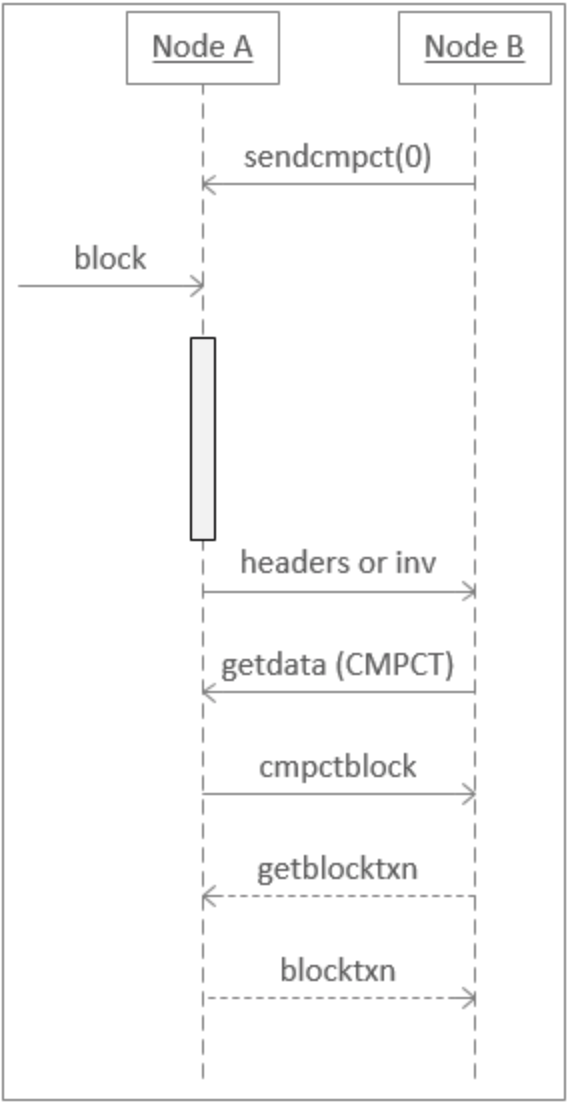
\includegraphics[width=.3\columnwidth, height=.4\columnwidth]{files/low_bandwidth_compact.png}
     \centering
     \caption{Low Bandwidth Compact Relay}
     \label{image: lowCompact}
\end{figure}

Bitcoin Improvement Protocol (BIP) 152 \citep{compact} introduces Compact blocks as a 
payload reduction technique. Compact blocks are based on the idea that most
transactions on the network are already transmitted to the peers and only the
difference in the information is to be sent across for efficient relay.

\begin{figure}
    \captionsetup{justification=centering}
    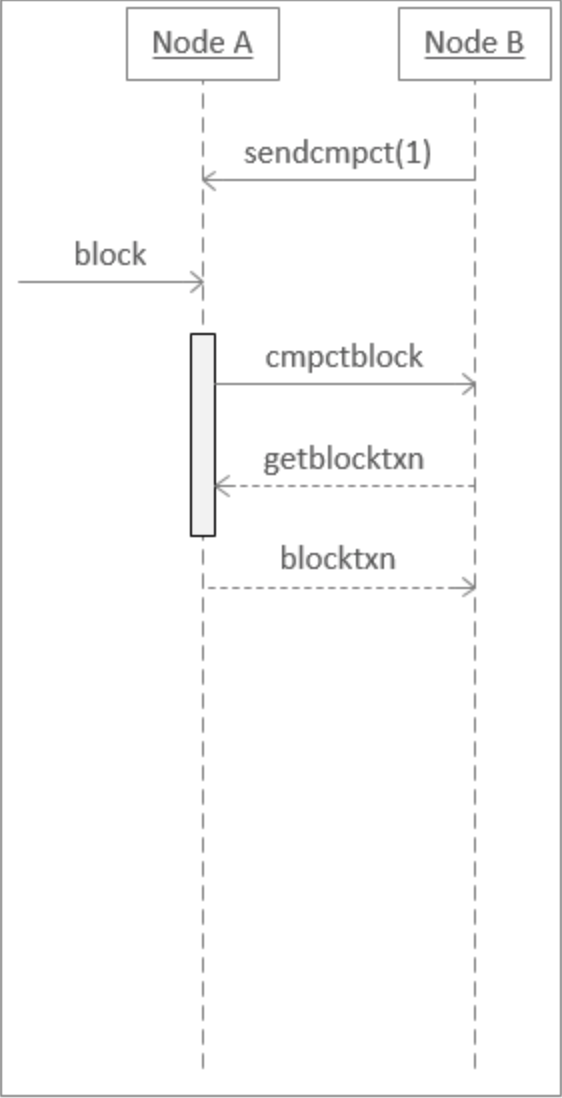
\includegraphics[width=.3\columnwidth, height=.4\columnwidth]{files/high_bandwidth_compact.png}
     \centering
     \caption{High Bandwidth Compact Relay}
     \label{image: highCompact}
\end{figure}


The process to relay a compact block is shown in \ref{image: highCompact} for high bandwidth relay and \ref{image: lowCompact} for low bandwidth compact relay and is explained below:


\begin{enumerate}
    \item
        All nodes that support compact blocks broadcast \texttt{Sendcmpct(0)} or
        \texttt{Sendcmpct(1)} for non-expedited or expedited relay respectively.
    \item 
        A new blocks is mined, the header or \texttt{inv} is sent to the receiving
        node.
    \item
        If the receiver node hasn't yet received the block, it sends a
        \texttt{getdata(cmpct)} request to the Sender node.
    \item
        The sender node responds with a compact block, which is collection of 6
        byte shortids of transactions and some pre-filled transactions that the
        node might not have heard of. (Example the coinbase transaction)
    \item
        In case of collision of the shortid or the receiver not having the
        transaction information, the peer requests all the transactions (it
        doesn't have) in the form of \texttt{getblocktxn} request.
    \item
        The above request is responded with a \texttt{blocktxn} message that
        contains the full transactions.
\end{enumerate}

Based on the above process, one can understand that the compact block saves
significant bandwidth by reducing the block payload to relay metadata
information across the network. \citep{compact-faq}  states that the maximum
sketch for a block is seen to be between 9 and 20KBs for 1MB block, and has a
90\% chance of block propagation happening without having to re-request the extra
transmissions. The protocol documentation does not provide any information on
how it affects when the block size increases or how this technique will scale
with an increased flow in transactions.  There are several weaknesses that were
observed after the protocol went live through a soft fork \citep{softfork}: 

\begin{enumerate}
    \item The memory pools of different nodes in a high transaction flow
        environment are not synchronized. The node allocates a certain amount of
        memory to its memory pool, and after this memory pool fills up, the
        transactions that arrive later are dropped

%    \item Birthday attacks (pigeon hole principle) can be constructed on the
%        block where 2 transactions of same short ID can be created. In this
%        case, the whole block is requested instead of the missing transactions.
%        This has been observed in attacks on nodes that were created by Peter
%        Schipper.

\end{enumerate}

\subsection{Xtreme Thin Block}

\begin{figure}
    \captionsetup{justification=centering}
    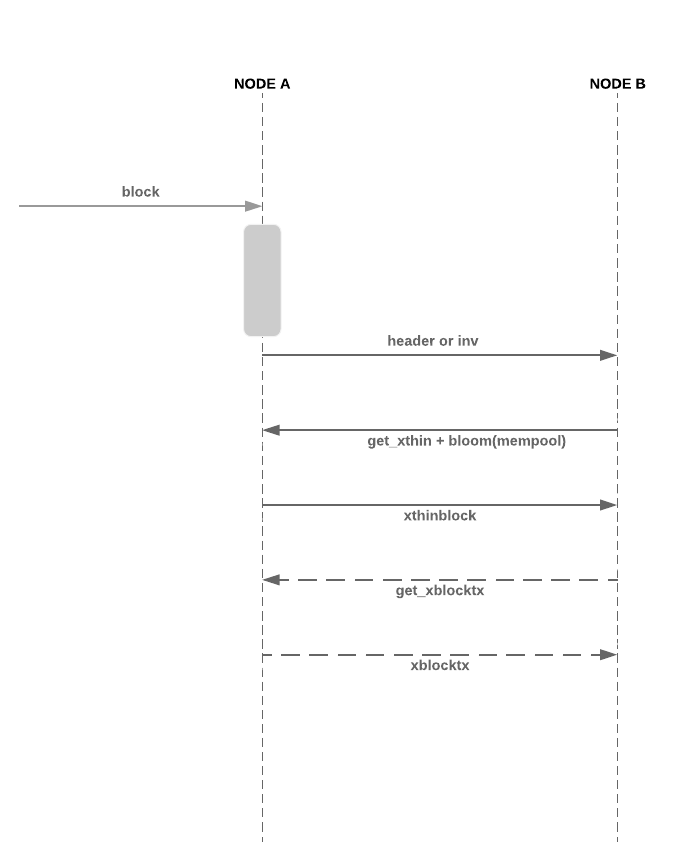
\includegraphics[width=.3\columnwidth, height=.4\columnwidth]{files/thinBlock.png}
     \centering
     \caption{XThin Relay}
     \label{image: xthin}
\end{figure}


Bitcoin Unlimited Improvement Protocol (BUIP010) \citep{buip10} proposed and implemented another
form of payload reduction called Extreme Thin Blocks \( XThin\). This technique uses a
similar technique as Compact block. It does add more complications explained
below in order to decrease the re-transmission rate.
The process to relay an XThin block is shown in \ref{image: xthin} and is explained below:


\begin{enumerate}
    \item
        All nodes that support XThin Blocks, run another service
        \texttt{NODE\_XTHIN} as a way of letting the network know the kind of
        blocks they support.
    \item 
        The receiver node creates a bloom filter of all the items in its memory
        pool. It then requests the block \texttt{getdata} along with the bloom
        filter.
    \item
        The Sender then sends the block adding all transaction IDs(8 bytes)
        also referred as cheap hashes along with header information and full transactions that the receiver
        doesn't have (based on the receiver's memory pool).
    \item
        The receiver reconstructs the block using the transactions that it has
        in its memory pool along with the full transactions supplied by the
        Sender.
\end{enumerate}

The protocol documentation states that the block sizes reduce to a maximum block
sketch of 17.5 KB in the experiments that were run on 1MB blocks. This was
observed when the protocol went live with Bitcoin-Bitcoin Cash hard fork as
well.

Xtreme Thin blocks face several problems as well:

\begin{enumerate}
    \item
        Bloom filters although encode information in a relatively much smaller
        size, but have a False Positive Rate associated with it. In case of of
        false positives, the full transactions are re-requested by the receiver
        node.
%    \item
%        The 8 byte transaction IDs do have collisions, although less than that
%        of Compact blocks. Collisions have been manufactured before on XThin
%        blocks, leading to Denial of Service attacks. For Dos prevention, on
%        collision, the thin block is re-requested which is a collection all 32
%        byte transaction IDs in the block.

\end{enumerate}

\subsection{Graphene blocks}

\begin{figure}
    \captionsetup{justification=centering}
    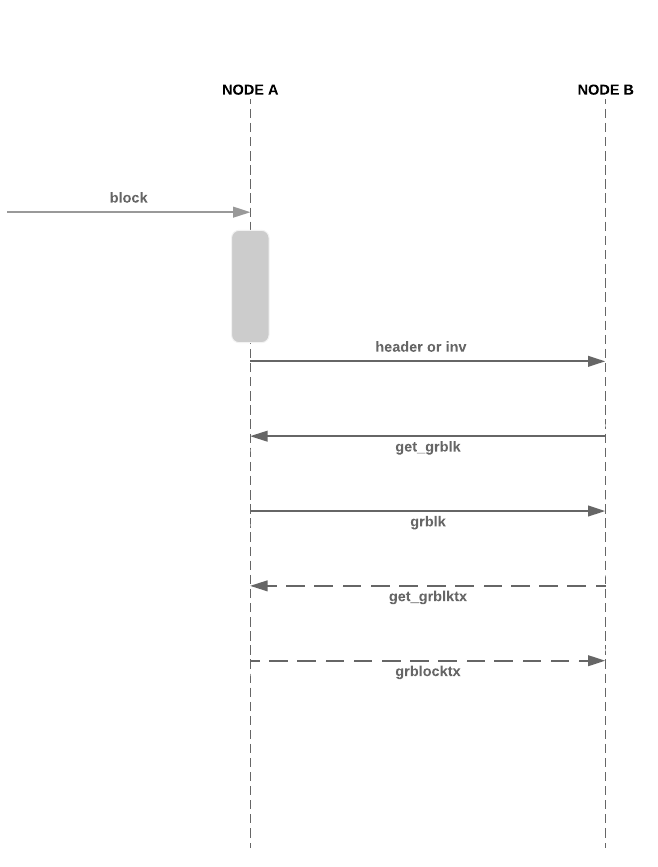
\includegraphics[width=.3\columnwidth, height=.4\columnwidth]{files/graphene.png}
     \centering
     \caption{Graphene Relay}
     \label{image: graphene}
\end{figure}

Bitcoin Unlimited Improvement Protocol (BUIP093) \citep{buip093} proposes Graphene Relay
propagation in order to further decrease the payload of a block. The Graphene
propagation however gets rid of the shortID list implementation and sends a
bloom filter along with an Invertible Bloom Lookup table \citep{iblt} in order to relay
information.

The graphene protocol is shown in \ref{image: graphene} and is explained below:

\begin{enumerate}
    \item The sender sends an \texttt{inv}:inventory message to notify an new
        block.
    \item The receiver requests the graphene block using \texttt{getgrblk}
        message along with the count of transactions in its mempool.
    \item The sender sends the graphene payload that consists of a bloom filter
        of all the transactions inside the block and an Invertible Bloom Lookup Table.
    \item The Invertible Bloom Lookup Table consists of a mapping of all
        transaction IDs along with the cheap hashes (the first 8 bytes of the
        Transaction ID).
    \item Ranks of transaction IDs are calculated using lexicographical ordering.
    \item The receiver on the other hand collects all transaction IDs in its
        memory pool and orphan pool and filters the transactions of the block
        using the Sender's bloom filter.
    \item Using these filtered transactions an IBLT is constructed at the
        receiver's end and subtracts the sender IBLT from it. 
    \item IBLT decode success is based on either the subtraction to lead an
        empty set or a non-empty set in which the remaining transactions can be
        requested again.
    \item IBLT decode failure can happen based on its probabilistic nature or
        when the receiver IBLT has very low transactions to match or a checksum
        failure.
\end{enumerate}

The above mentioned technique is highly efficient for sending large blocks when
memory pools are synced. In case of IBLT decode failures results in the node requesting a full block in order to avoid a Denial of Service attack.

\section{Current Proposal}

The techniques, mentioned in Section 1.2, 

\begin{enumerate} 
    \item rely on memory synchronization of nodes communicating the blocks and the overhead of decode failures is 
        re-transmission of full data back from the sender. 
    \item They also rely on a single
        peer to send the complete data as opposed to using multiple peers to transmit partial
        data. 
    \item They can only be used to receive blocks that are currently being propagated. They can't be used to sync new nodes. 

\end{enumerate}

\subsection{Digital Fountain}

This thesis aims to leverage the research of digital fountains 
\citep{fountain1} \citep{fountain2} \citep{fountain3} \citep{fountain4} in order to
propagate block information as a fallback method for the above existing
solutions.

In order to make these methods more efficient, this thesis aims to add a
protocol of aggregating data taken from multiple peer nodes in the form of encoded
symbols, collecting them over to the receiver end and re-constructing the block.

In case of block failure, in the current blockchains, the peer requests all the
full transactions from one peer using \texttt{getdata}. In case of large blocks, this is
a time consuming relay and can lead to higher orphan rates and hurt the
profitability of miners. As an alternative, the receiving node can request all
the peer nodes for part of data and reconstruct the block and recreate the
source block. This significantly reduces the uploads per peer in the network and
reduces the stress of data transmission per node. However, the overall data
downloaded by the receiving peer has some overhead in case of decode failures.

There are 2 ways of implementing this idea:

\begin{enumerate}
    \item Creating a list of transactions that are missing and dividing them
        among all nodes and requesting for the specific data.
    \item Requesting a Forward Error Correcting fountain code, that if the
        receiver has enough symbols of, can recreate the block. This method is
        explained and is worked out in this thesis.
\end{enumerate}

The reasons for using the latter technique are the following:

\begin{enumerate}
    \item The fountain code symbols can be transmitted over both UDP and TCP.
        While transmitting this data in a UDP network, there will be a need to
        transmit additional overhead symbols in case of data loss. 
    \item In a blockchain network, when in the above described techniques if a decode failure happens, the whole block data needs to be sent. However, when using fountain codes, the whole data need not be sent . It is sufficient to send more repair symbols to successfully decode. These symbols are
        smaller in size and, thus, get transmitted faster. 
    \item Miners with higher bandwidth can use asynchronous multicast to reliably transmit data.
\end{enumerate}

Trade offs of using the fountain code technique are as follows:

\begin{enumerate}
    \item Extra computation is added to a node in order to create the symbols
        before relaying them. These computations are only done once, by the miner while relaying the symbol. The other nodes can flush the symbols to disk and use it for relaying at anytime. 
    \item There is overhead while reconstructing the block. In order to
        decrease the number of decode failures, overhead repair symbols are
        added. However, this burden is added on the download side and not on
        upload side, because the upload is shared by a set of peers.
\end{enumerate}
